% **************************************************
% Document Class Definition
% **************************************************
\documentclass[%
  paper=A4,         % paper size --> A4 is default in Germany
  twoside=true,       % onesite or twoside printing
  openright,          % doublepage cleaning ends up right side
  parskip=full,       % spacing value / method for paragraphs
  chapterprefix=true,     % prefix for chapter marks
  11pt,           % font size
  headings=normal,      % size of headings
  bibliography=totoc,     % include bib in toc
  listof=totoc,       % include listof entries in toc
  titlepage=on,       % own page for each title page
  captions=tableabove,    % display table captions above the float env
  draft=false,        % value for draft version
]{scrreprt}%

% **************************************************
% Debug LaTeX Information
% **************************************************
%\listfiles

% **************************************************
% Information and Commands for Reuse
% **************************************************
\newcommand{\thesisTitle}{Implementation and Semantics of an asynchronous evaluation engine for stream based specifications}
\newcommand{\thesisName}{Alexander Schramm}
\newcommand{\thesisSubject}{Master Thesis}
\newcommand{\thesisDate}{November 20, 2016}
\newcommand{\thesisVersion}{My First Draft}

\newcommand{\thesisFirstReviewer}{Prof. Dr. Martin Leucker}
\newcommand{\thesisFirstReviewerUniversity}{\protect{University of Luebeck}}
\newcommand{\thesisFirstReviewerDepartment}{Institute For Software Engineering and Programming Languages}

\newcommand{\thesisSecondReviewer}{Who Knöws}
\newcommand{\thesisSecondReviewerUniversity}{\protect{University of Luebeck}}
\newcommand{\thesisSecondReviewerDepartment}{We will see}

\newcommand{\thesisFirstSupervisor}{Cesar Sanchez}
% \newcommand{\thesisSecondSupervisor}{John Smith}

\newcommand{\thesisUniversity}{\protect{University of Luebeck}}
% \newcommand{\thesisUniversityDepartment}{Institute For Software Engineering and Programming Languages}
\newcommand{\thesisUniversityInstitute}{Institute For Software Engineering and Programming Languages}
% \newcommand{\thesisUniversityGroup}{Clean Thesis Group (CTG)}
\newcommand{\thesisUniversityCity}{Luebeck}
\newcommand{\thesisUniversityStreetAddress}{Ratzeburger Allee 160}
\newcommand{\thesisUniversityPostalCode}{23562}

% **************************************************
% Load and Configure Packages
% **************************************************
\usepackage[utf8]{inputenc}   % defines file's character encoding
\usepackage[english]{babel} % babel system, adjust the language of the content
\usepackage[          % clean thesis style
  figuresep=colon,%
  sansserif=false,%
  hangfigurecaption=false,%
  hangsection=true,%
  hangsubsection=true,%
  colorize=full,%
  colortheme=bluegreen,%
  bibsys=bibtex,%
  bibfile=Mendeley,%
  bibstyle=alphabetic,%
]{cleanthesis}
\usepackage{amssymb}
\usepackage{amsmath}
\usepackage{tikz}
\usetikzlibrary{arrows.meta,decorations.pathmorphing,backgrounds,positioning,fit,petri}
\bibliography{Mendeley}
\cthesissetcolor{RGB}{0,75,90}{160,187,47}

\hypersetup{% setup the hyperref-package options
  pdftitle={\thesisTitle},  %   - title (PDF meta)
  pdfsubject={\thesisSubject},%   - subject (PDF meta)
  pdfauthor={\thesisName},  %   - author (PDF meta)
  plainpages=false,     %   -
  colorlinks=false,     %   - colorize links?
  pdfborder={0 0 0},      %   -
  breaklinks=true,      %   - allow line break inside links
  bookmarksnumbered=true,   %
  bookmarksopen=true      %
}

% **************************************************
% Document CONTENT
% **************************************************
\begin{document}

% --------------------------
% rename document parts
% --------------------------
%\renewcaptionname{ngerman}{\figurename}{Abb.}
%\renewcaptionname{ngerman}{\tablename}{Tab.}
\renewcaptionname{english}{\figurename}{Fig.}
\renewcaptionname{english}{\tablename}{Tab.}

% --------------------------
% Front matter
% --------------------------
\pagenumbering{roman}     % roman page numbing (invisible for empty page style)
\pagestyle{empty}       % no header or footers
% !TEX root = ../thesis-example.tex
%
% ------------------------------------  --> cover title page
% \begin{titlepage}
%     \pdfbookmark[0]{Cover}{Cover}
%     \flushright
%     \hfill
%     \vfill
%     {\LARGE\thesisTitle \par}
%     \rule[5pt]{\textwidth}{.4pt} \par
%     {\Large\thesisName}
%     \vfill
%     \textit{\large\thesisDate} \\
%     Version: \thesisVersion
% \end{titlepage}


% ------------------------------------  --> main title page
\begin{titlepage}
    \pdfbookmark[0]{Titlepage}{Titlepage}
    \tgherosfont
    \includegraphics[height=2.5cm]{gfx/isp-logo-english}\\
    \vfill

    % {\Large \thesisUniversity} \\[4mm]
    % \textsf{\thesisUniversityDepartment} \\
    % \textsf{\thesisUniversityGroup} \\

    {\centering
      {\LARGE \color{ctcolortitle}\textbf{\thesisTitle} \\[10mm]}
      {\large \thesisTitleGerman} \\
    }
    \vfill
    {\large \textbf{\thesisSubject}} \\[4mm]
    im Rahmen des Studiengangs\\
    {\large \textbf{Informatik}}\\
    der Universität zu Lübeck\\[7mm]
    vorgelegt von\\
    {\large \textbf{\thesisName}} \\

    \vfill
    \begin{minipage}[t]{.27\textwidth}
        \raggedleft
        \textit{ausgegeben und betreut von}
    \end{minipage}
    \hspace*{15pt}
    \begin{minipage}[t]{.65\textwidth}
        {\Large \thesisFirstReviewer} \\
    \end{minipage} \\[5mm]
    \begin{minipage}[t]{.27\textwidth}
        \raggedleft
        \textit{mit Unterstützung von}
    \end{minipage}
    \hspace*{15pt}
    \begin{minipage}[t]{.65\textwidth}
        {\Large \thesisFirstSupervisor} \\
      \end{minipage} \\[15mm]

      Die Arbeit ist im Rahmen einer Tätigkeit beim IMDEA Software Institute entstanden.\\[10mm]

    Lübeck, den \thesisDate \\

\end{titlepage}


% ------------------------------------  --> lower title back for single page layout
\hfill
\vfill

{
    \small
    \textbf{\thesisName} \\
    \textit{\thesisTitle} \\
    \thesisSubject, \thesisDate \\
    Reviewers: \thesisFirstReviewer \\
    Supervisors: \thesisFirstSupervisor \\[1.5em]%\ and \thesisSecondSupervisor \\[1.5em]
    \textbf{\thesisUniversity} \\
    % \textit{\thesisUniversityGroup} \\
    \thesisUniversityInstitute \\
    % \thesisUniversityDepartment \\
    \thesisUniversityStreetAddress \\
    \thesisUniversityPostalCode\ \thesisUniversityCity
}
    % INCLUDE: all titlepages
\cleardoublepage

\pagestyle{plain}       % display just page numbers
% !TEX root = ../thesis.tex
%
\pdfbookmark[0]{Abstract}{Abstract}
\chapter*{Abstract}
\label{sec:abstract}
\vspace*{-10mm}

This thesis studies the problem of software reliability using monitors specified with a stream runtime verification language.
In particular, we study the problem of evaluating specifications against finite streams of data.
The specifications we consider are written in the \gls{tessla} specification language, come from the field of Runtime Verification and describe correct behavior of running software systems.

Whether a run of a given system is correct is evaluated over trace data that is collected while the system is executing.
This data trace is represented as a collection of streams.
The specification states that this collection of input streams must fulfill specified conditions.

The first contribution of this thesis is the implementation of a \gls{tessla} evaluation engine, using an asynchronous and distributed approach to combine streams.
The engines we propose can check whether the traces produced by the running system satisfy the given specification.
The asynchronous nature of the engines we propose allows our solutions to scale to several parallel execution components for the evaluation engine.

The second contribution of this thesis is a proof of correctness of the implemented engines, based on the possible execution orders between the parallel asynchronous components.
We show that even the most asynchronous implementation produces the same verdicts as the ideal fully synchronize engine.



\clearpage

{\usekomafont{chapter}Abstract (Deutsch)}\label{sec:abstract-diff} \\

Diese Arbeit untersucht das Problem der Softwarezuverlässigkeit unter Nutzung von Monitoren, die mit einer strombasierten Runtime Verification sprache spezifiziert werden.
Im speziellen untersuchen wir die Auswertung von Spezifikationen über endliche Datenströme.
Die berücksichtigten Spezifikationen sind in der \gls{tessla} spezifikationssprache geschrieben, kommen aus dem Feld der Runtime Verification und beschreiben korrektes Verhalten von laufenden Softwaresystemen.

Ob ein Lauf eines gegebenen Systems korrekt ist wird über Tracedaten ausgewertet, die während der Ausführung des Programms gesammelt werden.
Diese Tracedaten werden als eine Menge von Datenströmen repräsentiert.
Eine Spezifikation verlangt, dass diese Menge von Datenströmen gegebene Bedingungen erfüllt.

Das erste Ergebnis dieser Arbeit ist die Implementierung eines \gls{tessla} Evaluierungs\-systems, welches einen asynchronen, verteilten Ansatz zur Kombination von Datenströmen benutzt.
Das System, welches wir vorstellen, ist in der Lage zu erkennen, ob die Tracedaten eines laufenden Systems eine Spezifikation erfüllen.
Die asynchrone Natur des Systems erlaubt es, das Evaluierungssystem auf mehrere, parallel ausführende Recheneinheiten zu skalieren.

Ein zweites Ergebnis dieser Arbeit ist ein Beweis der Korrektheit des implementierten Systems, basierend auf den möglichen Ausführungsreihenfolgen der parallel laufenden komponenten.
Wir zeigen, dass selbst ein maximal asynchron ausgeführtes System zu demselben Urteil, wie ein ideales, synchrones System, kommt.
    % INCLUDE: the abstracts (english and german)
\cleardoublepage
%
\input{content/acknowledgement} % INCLUDE: acknowledgement
\cleardoublepage
%
\setcounter{tocdepth}{2}    % define depth of toc
\tableofcontents        % display table of contents
\cleardoublepage

% --------------------------
% Body matter
% --------------------------
\pagenumbering{arabic}      % arabic page numbering
\setcounter{page}{1}      % set page counter
\pagestyle{maincontentstyle}  % fancy header and footer

% !TEX root = ../thesis.tex
%
\chapter{Introduction}
\label{sec:intro}

% \cleanchapterquote{You can’t do better design with a computer, but you can speed up your work enormously.}{Wim Crouwel}{(Graphic designer and typographer)}

\section{Motivation and Problem Statement}
\label{sec:intro:motivation}

Software verification is an important tool to harden critical systems against faults and exploits.
Due to the raising importance of computer based systems, verification has become a big field of research in computer science.

While pure verification approaches try to proof the correct behaviour of a system under all possible executions, \gls{rv} limits itself to single, finite runs of a system.
The goal is to proof that a run conforms to a given specification under specific conditions, like input sequences or scheduling.
Specifications can be given in various ways, e.g.\ as a \gls{tl} formula or in a specification language that is specifically developed for \gls{rv}.
Examples for this are \gls{rmor} \citep{Havelund2008}, \gls{lola} \citep{DAngelo2005} and others \citep{Zheng2015, Pike2010, Mostafa2015}, which we will look at more closely in \Cref{sec:related}.

The project \Gls{tessla}\citep{Decker2016} presents ways to specify and evaluate properties over streams of events including timing information.
To achieve this it introduces a language to expressively describe the conditions one or more streams should fulfill by applying transformations on them.
The evaluation of \gls{tessla} a specification is done in two steps: first the specification is compiled by a compiler written at the \gls{isp} of the University of Lübeck.
The output is a canonical representation of the transformations on the streams in the specification.
In the second step the compiled specification is connected with a system that produces traces that are treated as the input streams of the specification.

The second step can be done in different ways: online or offline, interweaving the monitors into the monitored program (like for example done in~\cite{Havelund2008}) or by executing them standalone.
These different approaches lead to different ways the monitored program has to be altered, e.g. manipulating its original code to log status informations or to invoke the monitoring code.

Interweaved monitors can alter the original system and produce new errors or even suppress others.
Standalone monitors on the other hand will have a much smaller impact on the monitored system.
But as a consequence there will be a bigger delay between the occurence of events in the program and their evaluation in the monitor.
Furthermore interweaved monitors can optionally react to detected errors.
They could change the control flow of the original system or alert a third party and eliminate cascading errors.
Standalone monitors can't directly modify the program but can still produce warnings and alerts that can then be reacted to.

While online monitoring can be used to actively react to error conditions, either automatically or by notification of a third party, offline monitoring can be thought of as an extension to software testing~\cite{DAngelo2005}.

At the beginning of this thesis there was one implementation of a runtime for \gls{tessla} specifications that is based on \glspl{fpga} that have to be manually reconfigured for each new specification.
While this is a very performant approach for actual monitoring it isn't feasible for testing and prototyping.
This leads to the wish to implement a software based \gls{tessla} runtime which can be executed independent of hardware restrictions.

Furthermore most \gls{rv} approaches are specific to one programming language or environment and combine ways of generating the data, which is used for monitoring, and the monitoring itself.
\gls{tessla} specifications themself are independent of any implementation details of the monitored system, working only on streams of data, which can be gathered in any way.
This can be used to implement a runtime that is also independent of the monitored system an how traces of it are collected.

During the thesis it is prooven that the actual approach of the runtime, a functional, actor based, asynchronous system, will generate the same observations on input traces as a synchronous evaluation of the specification.
While \gls{tessla} specifications can work on all kinds of streams, especially on traces on all levels of a program, e.g.\ on instruction counters or on spawning processes, in this thesis we will mainly focus on the level of function calls and variable reads/writes.
Other applications of the system could easily extend it to use traces representing drastically different fields, e.g.\ health data, temperatures, battery levels, web services and more.

To test the software based runtime different specifications will be tested on multiple traces.
Some of the traces are generated by actually running a program which was instrumented by hand or automatically to generate traces.
Others where are generated or modified by hand to deliberately introduce bugs which should be detected by the system.

\section{Results}
\label{sec:intro:results}

The main contributions of this thesis consist of three parts.
The first is a theoretical approach to asynchronously evaluate timed specifications over streams.
The second is an implementation that can synthesize systems to evaluate such specificationss based on the theoretical approach.
And the third is a proof of concept implementation of a system that can instrument code which is compiled with \gls{llvm}, mainly targeted at C and C++.
TODO: more


\section{Thesis Structure}
\label{sec:intro:structure}

As the whole evaluation engine is built on top of different technical and theroetical ideas, it is structured to show
the reasoning behind the decisions that were made during the development.
Furthermore it will proof equalitys of different kinds of systems in multiple steps that build on one another.
In the following a quick overview of the different parts of the thesis is given.

\textbf{\Cref{sec:related}}

In this chapter the theoretical foundation for the system is explained.
Furthermore multiple approaches solving similar problems are shown and it is highlighted which concepts of them were
used in the new system and which were disregarded and why.


\textbf{\Cref{sec:definitions}}

Building on the theoretical and practical findings of the previous chapters new definitions are presented, which are needed to reason about the implemented system.

\textbf{\Cref{sec:behaviours}}

The work from the previous chapter is put to work to reason about the semantics of the implemented runtime and to show its correctness.

\textbf{\Cref{sec:implementation}}

This chapter highlights technical details of the implementation.
It will present alternative implementation approaches and the reasoning why specific choices were made during the development of the system.

\textbf{\Cref{sec:evaluation}}

To show the value of the implemented system it is thoroughly tested and benchmarked with fabricated and real world examples and traces.
The results of this testing is used to evaluate the implementation.

\textbf{\Cref{sec:conclusion}}

On the basis of the evaluation in the conclusion the results of the thesis are summarized.
Furthermore it is highlighted what remains to do and which future challenges exist.


 % INCLUDE: introduction
% !TEX root = ../thesis.tex
%
\chapter{Related Work}
\label{sec:related}
\todo{Just a collection of thoughts for now, needs to be polished a lot}

% \cleanchapterquote{A picture is worth a thousand words. An interface is worth a thousand pictures.}{Ben Shneiderman}{(Professor for Computer Science)}
As Runtime Verification is a widely researched field there are many different approaches towards monitoring programs.
As stated in~\cite{Havelund2008} most approaches are geared towards Java, while many critical systems are written in C.
Because our implementation of a runtime is independent of the environment of the monitored program, this opens up the possibility to investigate this somewhat neglected field.
Therefore ways to generate traces from C programs are highlighted in this chapter.

TeSSLa itself and the implemented runtime builds on concepts and results of many other Runtime Verification techniques.
In the following sections some of them are highlighted to give a better understanding of choices made during this thesis.

\section{Distributed Verification Techniques}
\label{sec:related:distributed}

While most implementations of RV systems don't consider or use modern ways of parallelism and distribution and focus on programs running locally, in~\cite{Mostafa2015} a way to monitor distributed programs is given.
To do this distributed monitors, which have to communicate with one another, are implemented.

As stated earlier, the TeSSLa runtime doesn't care about the environment of the monitored program, so it doesn't distinguish between traces from distributed and non distributed programs.
But the runtime itself is highly concurrent and can be distributed easily to many processors or event different computers.
Therefore many of the definitions for distributed monitors can be used to reason about the behaviour of the Runtime.

\section{LOLA}
\label{sec:related:lola}

LOLA~\cite{DAngelo2005} has big influence on TeSSLa and the theoretical work of this thesis.
LOLA defines a very small core language to describe streams as the result of combinations on other streams.
In contrast to TeSSLa it is defined in regards of a discrete timing model.

Lola defines a notion of efficiently monitorable properties and an approach to monitor these properties.

TeSSLa takes concepts of LOLA and applies them to a continuous model of time and introduces a language and a rich
set of functions that can be applied to streams.

\section{Copilot}
\label{sec:related:copilot}

The realtime runtime monitor system Copilot was introduced in~\cite{Pike2010}.
Copilot is designed to overcome the shortcomings of existing RV tools in regards to hard-realtime software written in C.

To do so they first define characteristics a monitoring approach has to fullfill to be considered valuable for this domain.
The four principles are:

\begin{description}
  \item[Functionality] Monitors cannot change the functionality of the observed program unless a failure is observed.
  \item[Schedulability] Monitors cannot alter the schedule of the observed program.
  \item[Certifiability] Monitors must minimize the difficulty in re-validating the observed program; in particular, we make it our goal to avoid modifying the observed programs source code.
  \item[SWaP overhead] Monitors must minimize the additional overhead required including size, weight, and power (SWaP).
\end{description}

The monitors follow a sampling based approach, where at specified steps the values of global variables are observed and the monitors are evaluated
on that values.
While sampling based approaches are widely disregarded in RV, because they can lead to both false positives and false negatives,
they argue:

\begin{quote}
  In a hard real-time context, sampling is a suitable strategy. Under
  the assumption that the monitor and the observed program share a global clock and a static periodic schedule, while false positives are possible, false negatives are not.~\cite{Pike2010}
\end{quote}

A special detail of Copilot is that monitors aren't inlined into the program but can be scheduled as independet processes.
The implementation of the TeSSLa runtime in this thesis follows a similar approach: It is a totally independent program,
and therefore also has some of the gains in regard to the specified four characteristics.
Because the runtime works with all kinds of traces, it is insignificant how they are produced:
It can work with traces based on sampling, working in a similar fashion as Copilot, or by actually instrumenting code to generate
traces, which alters the semantics of the program.

% Another shortcoming of inlining monitors is that certified code (e.g., DO-178B for avionics [Inc92]) is common in this domain.
% Inlining monitors could necessitate re-certifying the observed program.

\section{RMoR}
\label{sec:related:rmor}

RMoR is another approach on monitoring C programs.
It does so by transforming C code into an \emph{armored} version, which includes monitors to check conformance to a specification.

Specifications are given as a textual representation of state machines.
The specifications are then interweaved into the programm using CIL~\cite{Necula2002}.
Specifications work on the level of function calls and state properties like \emph{write may never be called before open was called}.
Because Software Developers are often working at the same abstraction level (in contrast to e.g.\ assembler or machine instructions), they can define specifications without having to learn new concepts.
For the TeSSLa runtime support for traces at the same abstraction level (function calls, variable reads and writes) is present and used in most of the tests in Section~\ref{TODO}.

Because RMoR specifications are interweaved into the program, their observations can not only be reported but also used to recover the program or even to prevent errors by calling specified functions when some condition is encountered.
The TeSSLa runtime doesn't support this out of the box, as it's primary purpose is testing and offline monitoring, but in Section~\ref{TODO:Further_WORK} we will look at ways to support this.

% \section{Driver Trace}
% \label{sec:related:drivertrace}
\section{MaC}
% \section{RiTHM}
 % INCLUDE: related work
% !TEX root = ../thesis-example.tex
%
\chapter{System}
\label{sec:system}

\section{Evaluation Engine}
\label{sec:system:eval_engine}

\subsection{Erlang and Elixir}
\label{sec:system:eval_engine:erlang_elixir}
todo: BEAM, Actors/Thread, multiplattform (nerves project)

\subsection{Implementation}
todo: Timing model: reason why events have to carry timestamps in contrast to interweaved monitors

\section{Trace Generation}
\label{sec:system:traces}

\subsection{TraceBench}
\subsection{Aspect oriented programming}
\subsection{CIL}
\subsection{Google XRay}
\subsection{GCC instrument functions}
\subsection{Sampling}
\subsection{LLVM/clang AST matchers}
 % INCLUDE: system
% % !TEX root = ../thesis-example.tex
\chapter{Concepts}
\label{sec:concepts}

In this Chapter different ways to evaluate TeSSLa specifications are given and their equivalence is shown.
To do so in Section~\ref{sec:concepts:defs} building blocks for evaluation approaches are defined, which are then used in later Sections to define behaviour of them and show their equivalence.

\section{Definitions}
\label{sec:concepts:defs}

While the TeSSLa specification itself defines a set of semantics, for this Thesis we will slightly alter some of it and add some new definitions based on them.
This is necessary to reason about the specifics how the evaluation engine is built (Note that TeSSLa doesn't define an operational semantic, therefore we will define our own) and how it behaves.

\subsection{Time}
\label{sec:concepts:defs:time}

TeSSLa has a model of continuous Time, where timestamps \(t \in \mathbb{T} \) are used to represent a certain point in Time and \(\mathbb{T}\) has to be isomorphic to \(\mathbb{R}\).

\subsection{Events}
\label{sec:concepts:defs:events}

Events are the atomic unit of information that all computations are based on.
There are three Types of Events: input, output and internal Events.

The Set of all Events is denoted as \(E\).
Each event carries a value, which can be \emph{nothing} or a value of a Type (types are formally defined in the TeSSLa speicification but aren't important for this thesis), a timestamp and the stream it's perceived on (e.g.\ a function call of a specific function or the name of an output stream).

The value of an event can be queried with the function \(\upsilon\), its timestamp with \(\pi\) and its Stream with \(\varsigma\).

\(E_i \subset E\) is the Set of all input events, their Stream corresponds to a specific trace.
\(E_o \subset E\) is the Set of all output events, their Stream is specified by an output name of the TeSSLa specification.
\(E_n \subset E\) is the Set of all internal events.
Internal events are mostly an implementation detail, which denote steps of computation inside the runtime.
The Stream of internal events is implicitly given by the node that produces the stream of the Event.
Note that \(E_i, E_o, E_n\) are pairwise disjoint and \(E_i \cup E_o \cup E_n = E\).

\subsection{Streams}
\label{sec:concepts:defs:streams}

Streams are a collection of Events with specific characteristics.
While Events are the atomic unit of information, Streams represent the sequence of related Events over time.

There are two kind of Streams: Signals, which carry values at all times, and Event\-streams, which only hold values at specific times.
EventStreams can be described by a sequence of Events.
Signals can be described by a sequence of changes, where a change denotes that the value of a Signal changed at a specific timestamp.
The only difference between a Signal and an EventStreams is that Signals always have a value while an EventStream may return \(\bot\) when queried for its value at a specific time, which denotes, that no event happened at that time.
Based on the similarity of Signals and Eventstreams in the following we will mainly reason about Eventstreams, but most things can also be applied to Signals.

Formally a Stream \(\sigma\) can be represented as a Sequence of Events \(\langle e_1, \dots e_n\rangle\) where \(\pi(e_i) < \pi(e_{i+1}),\ \forall i < n \in \mathbb{N}\).
The Set of all Streams \(\Sigma\) is defined as all possible finite sequences of Events \(\Sigma = \{\sigma | \sigma \in E^* \}\).
An input Stream \(\sigma_i\) is a stream consisting only of input Events, the set of all input Streams is \(\Sigma_i = \{\sigma_i | \sigma_i \in E_i^*\}\).
Output and internal Streams are defined analogous.
To get the Event of a Stream \(\sigma\) at a timestamp \(t\) it can be queried like a function: \(\sigma(t) = e\) with \(\pi(e) = t \).
When working with Signals, the function will return the latest Event that happened at or before t while an EventStream may return \(\bot\).

Furthermore Streams hold the timestamp to which they have progressed, which can be equal or greater than the timestamp of the last Event happened on them.
The progress of a Stream can be obtained with \(p(\sigma) = t \in T\).

Internal and output Streams can be queried for the Node that produced them with \(\eta(\sigma) = n \in N\).

\subsection{Transducers}
\label{sec:concepts:defs:transducers}

Fundamentally TeSSLa is a special kind of a Transducer.
Therefore in this Section we will define a model of Transducers which can be used to reason about the evaluation of a TeSSLa specification.

A Transducer is a System, which consumes an input and produces an output.

\begin{definition}[name = Transducer]\label{def:transducer}
  Let \(\Phi, \Gamma\) be two Alphabets.
  A Transducer \(t\) is a Relation \(t \subseteq \Phi^* \times \Gamma^*\), \(\Phi\) is called the input Alphabet, \(\Gamma\) the output Alphabet.
\end{definition}

TeSSLa specifications are deterministic for any input, meaning they should produce the same output for the same input.

\begin{definition}[name = Deterministic Transducer]\label{def:deterministic_transducer}
  A deterministic Transducer relates each input to at most one output.
\end{definition}

Transducers can furthermore be categorized as synchronous, asynchronous, causal and clairvoyant Transducers:
Synchronosity is a property over the behaviour of a Transducer when it's consuming input per element.
If it is synchronous, it will produce an output element for each input element.

\begin{definition}[name = Synchronous Transducer]\label{def:synchronous_transducer}
Let \(\vec{\imath} \in \Phi^*, i \in \Phi, \vec{o} \in \Gamma^*, o \in \Gamma\).
  A Transducer \(t\) is called synchronous, when it satisfies the formula:
  if \( (\vec{\imath}\circ i,\vec{o}\circ o) \in t\)
  then \( (\vec{\imath}, \vec{o}) \in t \)
\end{definition}

An asynchronous Transducer can produce zero, one or many outputs for each input it consumes.

\begin{definition}[name = Asynchronous Transducer]\label{def:asynchronous_transducer}
  Let \(\vec{\imath}\in \Phi^*, i \in \Phi,\vec{o} \in \Gamma^*\).
  A Transducer \(t\) is called asynchronous when it satisfies the formula:
  if \((\vec{\imath}\circ i, \vec{o}) \in t \)
  then \(\exists \vec{o'},\vec{o''} \in \Gamma^*\text{ so that } \vec{o} = \vec{o'}\circ\vec{o''} \text{ and } (\vec{\imath},\vec{o'}) \in t \)
\end{definition}

A causal Transducer is one, where the output depends only on consumed inputs and not on future inputs:

\begin{definition}[name = Causal Transducer]\label{def:causal_transducer}
  A Transducer \(t\) is called causal, when it satiesfies the condition:
  if \((\vec{\imath},\vec{o}) \in t \)
  then \( \forall \vec{\imath'} \in \Phi^* \text{ with } (\vec{\imath} \circ \vec{\imath'}, \vec{o'}) \in t \)
  it holds, that \( \vec{o} \sqsubseteq \vec{o'} \)
\end{definition}

A Transducer that isn't casual is called \emph{clairvoyant}.

When talking about Transducers, it is interesting to know if two Transducers are \emph{equivalent}.
There are multiple possible definitions for equivalence of Transducers, we will look at two, which are interesting for this thesis.

\begin{definition}[name = Asynchronous equivalence of Transducers]\label{def:async_equivalence_transducer}
  Let \(t_1, t_2\) be two asynchronous Transducers from \(\Phi^*\) to \(\Gamma^*\).
  They are called \emph{asynchronous equivalent}, written \(t_1 \equiv_a t_2\): \\
  if \(\forall (\vec{\imath},\vec{o}) \in t_1\) \\
  then \( \forall \vec{\imath'} \in \Phi^*, \vec{o'} \in \Gamma^* \text{ such that } (\vec{\imath}\circ\vec{\imath'},\vec{o}\circ\vec{o'}) \in t_1\) \\
  it holds, that \( \exists k,j \in \mathbb{N} \text{ with  } \vec{\imath_k} = (\vec{\imath}\circ\vec{\imath'}_{[0,k]}),
  \vec{o_j} = (\vec{o}\circ\vec{o'}_{[0,j]}) \text{ and } (\vec{\imath_k}, \vec{o_j}) \in t_2\)
\end{definition}

For the second kind of equivalence we need to introduce \emph{timed Transducers}.

\begin{definition}[name = Timed Transducer]\label{def:timed_transducer}
  Let \(\mathbb{T}\) be a timing model that is isomorphic to \(\mathbb{R}\).
  A timed Transducer \(t\) works on timed inputs and produces timed outputs:
  \[t \subseteq {\left(\Phi \times \mathbb{T}\right)}^* \times {\left(\Gamma \times \mathbb{T}\right)}^*\]
\end{definition}

The Function \(\text{timed:} {(\Gamma \times \mathbb{T})}^* \rightarrow {(\Gamma \times \mathbb{T})}^* \)
reorders a timed output sequence \(\vec{o}\) by its timestamps, such that:
\[
  \forall i,j \in \mathbb{N}:\text{ if } i < j \text{ then } t_i < t_j \text{ with } (o_i, t_i) = \vec{o}_i \text{ and } (o_j, t_j) = \vec{o}_j
\]

Based on this function, timed Transducers can be compared with respect to the timestamp of its output:

\begin{definition}[name = Observational Equivalence]\label{def:observational_equivalence}
  Two timed Transducers \(t_1, t_2\) are called observational equivalent, written \(t_1 \equiv_o t_2\),\\
  if \(\forall (\vec{\imath},\vec{o}) \in t_1\) \\
then \( \forall \vec{\imath'} \in {(\Phi\times\mathbb{T})}^*, \vec{o'} \in {(\Gamma\times\mathbb{T})}^* \text{ such that } (\vec{\imath}\circ\vec{\imath'},\vec{o}\circ\vec{o'}) \in t_1\) \\
it holds, that \( \exists k in \mathbb{N},j \in \mathbb{N}_{\geq\text{length}(\vec{o})} \text{ with  } \vec{\imath_k} = (\vec{\imath}\circ\vec{\imath'}_{[0,k]}),
  \vec{o_j} = (\vec{o}\circ\vec{o'}) \text{ and } (\vec{\imath_k}, \vec{o_j}) \in t_2\)
\end{definition}

% \begin{definition}[name = Timed Function]\label{def:timed_function}
%   Let \(\vec{o},\vec{o'} \in {(\Gamma \times \mathbb{T})}^*, (o_1, t_1), (o_2, t_2) \in {(\Gamma \times \mathbb{T})}, t_1 \neq t_2\).
%   Then:
%   \begin{align*}
%     &\text{timed}((o_1, t_1)) &&= (o_1, t_1) \\
%     &\text{timed}((o_1, t_1)\circ (o_2, t_2)) &&=
%     \begin{cases}
%       (o_1, t_1)\circ (o_2, t_2) \text{, if } t_1 < t_2 \\
%       (o_2, t_2)\circ (o_1, t_1) \text{, else}
%     \end{cases} \\
%     &\text{timed}(\vec{o}\circ(o_1,t_1)\circ\vec{o'}) \text{, } t_1 \text{ has the smallest time of all elements in } \vec{o}, \vec{o'} = (o_1,t_1)\circ\text{timed}(\vec{o}\circ\vec{o'})
%   \end{align*}
% \end{definition}


\subsection{Functions}
\label{sec:concepts:defs:functions}

A TeSSLa specification consists of Functions.
Functions generate new Streams by applying an operation on other Streams.
TeSSLa itself defines a syntax to write a specification, a set of types and a standard library of Functions, but an implementation is free to choose the functions it supports.

An example Function is \(add(S_D,S_D) \rightarrow S_D\): It takes two Signals, which have to hold values of some numerical type, and produces a signal which holds values of the same type.
The produced stream can either be assigned to a named identifier (think: a variable) or consumed by another function (function composition).

Functions can be divided into three categories: pure, unpure and timing.
Pure Functions, also called stateless, are evaluated only on the values their inputs have at the timestamp they are evaluated, therefore they don't have to \emph{remember} anything about earlier Events.
Unpure, or stateful, Functions are evaluated over the whole input Stream, meaning they can look at all Events that happened on its inputs before the time of evaluation and also at all it's previous output Events.
E.g.\ a Function \emph{eventCount} has to \emph{remember} how many events already happened on it's input stream and increment that counter on every new event.
Timing Functions are evaluated not only on the value of Events but also on their timestamp and can also manipulate it:
While non timing Functions will consume events at a specific timestamp and emit an event with that timestamp, timing functions can emit Events with a different timestamp.

Timing Functions complicate the reasoning about schedules and causality and therefore aren't included in Section~\ref{sec:concepts:behaviour_without_timing}.
In Section~\ref{sec:concepts:behaviour_with_timing} the conclusions of earlier sections will be extended to include timing Functions.


\subsection{Nodes}
\label{sec:concepts:defs:nodes}

Nodes are the atomic unit of computation for the evaluation of a TeSSLa specification.
A Node implements a single Function, e.g.:\ there is an \emph{AddNode} which takes two input Signals and produces a new Signal.
Therefore a Node is the concrete implementation of a Function in a runtime for TeSSLa specifications.
The set of all Nodes is called \(N\).
The Function of a Node \(n \in N\) is written as \(f_n\).

Each Node has a set of inputs, which are either input or internal Streams, and one output, which is either an internal or an output Stream.
Nodes use a FIFO queue, provided by the Erlang plattform, to process new received Events in multiple steps:

\begin{enumerate}
  \item Add the new Event to the inputs
  \item Check if a new output Event can be produced (see Section~\ref{sec:concepts:defs:nodes:processable})
  \item If so, compute all timestamps, where new Events might be computed and
    \begin{enumerate}
      \item Compute the Events, add them to the History as new outputs
      \item Distribute the updated output to all successors
    \end{enumerate}
  \item Else wait for another input
\end{enumerate}

\subsubsection{Determination of processable Events}
\label{sec:concepts:defs:nodes:processable}

Based on the asynchronous nature of Nodes, Events from different Streams can be received out of order.
E.g.\ if a Node C is a child of Node A and B, it can receive Events from Node A at timestamps \(t_1, t_2, t_3, t_4\)
before receiving an event with timestamp \(t_1\) from Node B.
Therefore a Node can not compute it's output upto a timestamp unless it has informations from all predecessors that they did progress to that timestamp.
When Node C receives the first four Events from Node A, it will only add them to it's inputs but won't compute an output.
When it finally receives the first Event from Node B it can compute all Events upto \(t_1\).
To do so it will compute \emph{change timestamps}: The union of all timestamps where an Event occured on any input between the timestamp of the last generated output and the minimal progress of all inputs.

To see why this is necessary lets assume that Node C will receive a new Event from Node B with timestamp \(t_4\):
All inputs have progressed to \(t_4\), but on the Stream from Node A there are changes between \(t_1\) (where the last output was generated) and \(t_4\),
therefore the \emph{change timestamps} are \(t_2, t_3, t_4\) and the Node will have to compute it's output based on the values of the streams at that timestamps.

\subsection{TeSSLa Evaluation Engine}
\label{sec:concepts:def:eval_engine}

Because Functions in TeSSLa specifications itself depend on other Functions, and these dependencies have to be circle free,
the specification can be represented as a DAG@.
This DAG can be directly translated into an evaluation Engine for that specification: The Nodes of the DAGs are Nodes representing the functions and the Edges are the input and output Streams between the Nodes.

\begin{definition}[name=Equivalence of evaluation Engines]\label{def:equivalence_eval_engine}
  Two evaluation Engines are called equivalent, if they produce the same relationship between inputs and outputs for all possible inputs.
\end{definition}

\begin{definition}[name=Equivalence of evaluation Engines for an input]\label{def:equivalence_eval_engine_specific}
  Two evaluation Engines are called equivalent for an input, if they produce the same output for that input.
\end{definition}

To evaluate a specification over Traces, the Evaluation Engine has process the Events that were traced.
To do so the Nodes have to run their computations until no more Events are present (or the specification found an error in the trace).
This leads to the question in which order Nodes should be scheduled to perform their computation.
While some schedules are simply not rational (think of unfairness and causality) there are many different schedules that are feasible.
It has to be prooven that a chosen schedule produces the correct conclusions for a specification, else the evaluation Engine is not valid.

In this Thesis it is shown that multiple schedules will lead to the same conclusions and therefore an implementation of an evaluation Engine is free to choose between them.

\subsection{State and History}
\label{sec:concepts:def:state}

All TeSSLa evaluation Engines have to hold a State, which encodes information necessary to continue the evaluation, and a History, which encodes what happened on all Streams in the evaluation Engine.
The State of a whole evaluation Engine is made up of the States of its Nodes.

Each Node has a State, which can hold arbitray information, e.g.\ a counter for a \emph{CountNode}, and its input queues.
Input queues are Fifo queues, which hold the Events produced by predecessors of the Node, that weren't consumed yet by the Node.
% Each Node has a State which holds the History of its input Streams and its output Stream.
% One part of the State of every Node is the History of a Node, which holds all Events received from it's parents, called it's inputs, and all produced Events of the Node, called it's output.

To distinguish between the two types of States, we will call the State of the whole Engine the \emph{global State} and the State of a Node the \emph{Node State}.
The Set of all valid node States is called \(\widetilde{N}\).

% Formally the State of a Node is a  Set of a Sequence of the inputs (which are internal or input Streams) and the output (an internal or an output Stream).
% The Set of all valid Node States \(\widetilde{N} = {(\Sigma_i \cup \Sigma_n)}^*\times(\Sigma_n \cup \Sigma_o)\).

The global State of an evaluation Engine at a certain step is a map from its Nodes to their node State.
We will call the Set of all global States as \(S\).
A global State can be queried like \(s(n) = \widetilde{n}\) to yield the State of the Node \(n\).

Everytime a Node \(n\) is scheduled, it changes its own node State and the node State of its direct children \(N_c\) by

\begin{itemize}
  \item Take one Event \(e_i\) from each input queue \(q_i\): \(e_i = hd(q_i)\)
  \item Produce new Events based on the internal information and the taken Events
  \item Change its children node State by appending the produced Events to the queues of all Nodes in \(N_c\)
  \item Update its own node State by
  \begin{itemize}
    \item Updating the internal information if necessary
    \item Replace all input queues \(q_i\) with \(q_i' = tl(q_i)\)
  \end{itemize}
\end{itemize}

TODO History

\subsection{Transitions}
\label{sec:concepts:def:transitions}

A Transition describes what happens when the evaluation Engine switches State by performing a Step:
The consumption of one Event from each input of a Node and the optional generation of one or more new output Events of that Node.
To look at it in another way: A Transition is the computation of a Node, therefore when we say `Node A is scheduled' we mean that a Transition is taken which models the computation of that Node.

Formally Transitions are a Relation between two Sets of Events.
E.g.\ the Transition \(\tau = (\{e_1,e_2\}, \{e_3\})\) specifies that two Events were consumed by a Node (thereby adding them to its inputs) and one Event was produced based on them (which is added to the output).
The Set of all Transitions is
\begin{align*}
  T = \{(e, e') | &e \subseteq (E_i \cup E_n) \land e \neq \emptyset \land e' \subseteq (E_n \cup E_o)\\
                  &\land (\forall e_i, e_j \in e': \varsigma(e_i) = \varsigma(e_j)) \land (\forall \widetilde{e}_i, \widetilde{e}_j \in e: \varsigma(\widetilde{e}_i) \neq \varsigma(\widetilde{e}_j)\}
\end{align*}
where the Node which caused the Transition is \(\eta(\varsigma(e_i))\).
For brevity we define \(\eta : T \rightarrow N\) with \(\eta((e, e') = \eta(\varsigma(e_i)),\ e_i \in e'\), which yields the Node that is modeled by the Transition.

The empty Transition, meaning no input was consumed and no output produced, is labeled with \(\lambda\).
Note that all Transitions, except the empty one, have to consume at least one Event (therefore no Events can be created from nowhere) and that it's possible that no Event was produced based on the consumed Events (think of a \emph{FilterNode}).
Furthermore it's theoretically possible to create multiple Events in one Transition.
This makes only sense in the context of Timing Nodes, because else the generated Events would have the same timestamp, which is forbidden by the definition of Streams.
With Timing Nodes one could for example implement an \emph{EchoNode}, which duplicates an input after a specified amount of Time.

\begin{definition}[name = Application of a Transition on a State]\label{sec:concepts:def:application_transition}
  Given a global State \(S_0\) and a Transition \(\tau_1 = (e, e') = (\{e_1,e_2,\dots,e_i\}, \{e_1',e_2',\dots,e_i'\})\), when we \emph{apply} \(\tau_1\) to \(S_0\) we get a new global State \(S_1\) with\\
  \(\forall \widetilde{n}_i = S_0(i)\)
  \begin{itemize}
    \item if \(\eta(\widetilde{n}_i) \neq \eta(\tau_1) \rightarrow S_1(i) = \widetilde{n}_i\) (No Node States changes except the one from the Node of the Transition)
    \item else let \((\{\sigma_1,\dots,\sigma_n\}, \sigma_o) = n_i\). Than is \(S_1(i) = (\widetilde{\sigma}, \sigma_o')\) with
      \begin{itemize}
        \item \(\sigma_o' = \sigma_o ++ e'\) with \(++\) defined as appending all Events in \(e'\) to \(\sigma_o\) ordered by their timestamp
        \item \(\widetilde{\sigma} = \{\sigma_1', \sigma_2', \dots, \sigma_n'\}\) with \(\sigma_l', l \in [1,n]: \sigma_l + \widetilde{e}\) where \(\widetilde{e} \in e \land \eta(\varsigma(\widetilde{e})) = \eta(\sigma_l)\) and \(+\) is the known append operator for sequences.
      \end{itemize}
  \end{itemize}

\end{definition}
This means, that the new global State is built with the old global State by altering only the Node State of the Node identified by the Events in the second element of the Transition.
The Node State is altered by appending all Events in the second Element of the Transition to the output ordered by their timestamp and by adding each Event in the first element of the Transition to the input corresponding to the Stream of that Event.

\subsection{Run}
\label{sec:concepts:def:run}

A Run of an evaluation Engine is a sequence of Transitions and States.
The first element of the sequence is the empty Transition and the initial State of the evaluation Engine.
It is a representation of the steps the Engine takes to evaluate a specification over input Streams.
The length of a Run can be retrieved with \(l(R_1) = d \in \mathbb{N}\).
A Run can be queried by it's index to return the element at that index: \(R_1(i)=(\tau_i, S_i),\ i \in [0, l(R_1)]\).

The Run \(\langle (\lambda, s_0), (\tau_1, s_1) \rangle\) means, that the Engine was in it's initial State, took the transition \(\tau_1\) and thereby reached the state \(s_1\).

\begin{definition}[name = Equivalence of Runs]\label{def:equivalence_runs}
  Two Runs are called equivalent if they have an equal State at their last position.
\end{definition}

Because the State can be built from the Transitions that were taken, equivalence can also be defined over Transitions.

\begin{lemma}[name = Equivalence of Runs over Transitions]\label{lemma:equivalent_runs_with_transitions}
  If the Set of Transitions of two Runs are equal, the Runs are equivalent.
\end{lemma}

\begin{proof}
  Let \(R_1, R_2\) be the Runs of two Engines with the same Set of Transitions \(T'\).
  Let \(S_1\) be the final State of the Run \(R_1\) and \(S_2\) of \(R_2\).
  If the two global States weren't equal, there would have to be at least one \(i\) with \(S_1(i) \neq S_2(i)\), meaning the same Node has to have a different State in both Engines.
  Let \(\widetilde{n}_1, \widetilde{n}_2\) be the Node States of one such Node in both Engines.
  If the two Node States are different, one of them has to contain at least one Event on an input or output that isn't on the same Stream in the other State.
  Let that Event be \(e_d\).
  To be added to the State, there has to be a Transition \(\tau = (e, e')\) with \(e_d \in e \lor e_d \in e'\).
  This Transition has to be in \(T'\), which means it was taken by both Engines, therefore \(e_d\) is in the History of the Node in both Runs, therefore its the two Node States are equal in both Engines.
\end{proof}

\begin{definition}[name = Distance of Runs]\label{def:runs_distance}
  The Distance \(\delta\) of a Run \(R_1\) to a Run \(R_2\) is a pair \(\delta(R_1,R_2) = (x,y)\), where \(x\) is the index before the first position where the two Runs differ and y is the number of Steps between the index of the first difference and the position where \(R_2\) takes the Transition that \(R_1\) took after step \(x\).
  The Distance of Runs is ordered element-wise: \((x,y) < (x',y') \leftrightarrow ((x > x') \lor (x = x' \land y < y))\).
  Therefore two Runs with length \(d\) are equal, if their Distance is \(d,0\), which is the minimal Distance two Runs of length \(d\) can have at all.
\end{definition}

\begin{exmp}
  Let
  \[R_1 = \langle (\lambda, S_0), (\tau_1,S_1), (\tau_2,S_2), (\tau_3,S_3), (\tau_4,S_4), (\tau_5,S_5), (\tau_6,S_6) \rangle\]
  \[R_2 = \langle (\lambda, S_0), (\tau_1,S_1), (\tau_2,S_2), (\tau_5,S_3'), (\tau_4,S_4'), (\tau_6,S_5'), (\tau_3,S_6') \rangle\]
  \[R_3 = \langle (\lambda, S_0), (\tau_1,S_1), (\tau_2,S_2), (\tau_3,S_3), (\tau_5,S_4''), (\tau_4,S_5''), (\tau_6,S_6'') \rangle\]

  Than is
  \[\delta_{1,2} = \delta(R_1,R_2) = (3,3),\ \delta_{1,3} = \delta(R_1,R_3) = (4,1)\]
  \[\delta_{2,1} = \delta(R_2,R_1) = (3,2),\ \delta_{2,3} = \delta(R_2,R_3) = (3,1)\]
  \[\delta_{3,1} = \delta(R_3,R_1) = (4,1),\ \delta_{3,2} = \delta(R_3,R_2) = (3,2)\]

  And \(\delta_{1,3} < \delta_{2,3} < \delta_{2,1} < \delta_{2,1}\).


\end{exmp}

\begin{definition}[name = Enabledness of a Node]\label{def:node_enabled}
  A Node \(n\) with the input Streams \(\widetilde{\sigma}\) in an evaluation Engine is called \emph{enabled} at a Step \(s\) of a Run \(R_1\) of that Engine, when it satisfies all of the following conditions:

  \begin{itemize}
    \item All consumed Events are either internal Events that were produced at an earlier step or external Events that are present:
      \begin{itemize}
        \item \(\forall \sigma_x \in \widetilde{\sigma} \cap \Sigma_n: \exists j \in [1, s]: R_1(j) = (\tau_j, S_j)\) with
          \begin{itemize}
            \item\( (e, e') = \tau_j \land e_x \in e'\) with \(\varsigma(e_x) = \sigma_x \)
          \end{itemize}
        \item and \(\forall \sigma_i \in \widetilde{\sigma} \cap\Sigma_i:\exists e_i\) with \(\varsigma(e_i) = \sigma_i\)
      \end{itemize}
    \item and weren't consumed earlier by that Node
      \begin{itemize}
        \item \(\forall e_x\) (the same \(e_x\) as in the steps above)
          \begin{itemize}
            \item \(\not\exists h \in [j, s]: (\widetilde{e}, \widetilde{e'}) = \tau_h \land \eta(\tau_h) = n \land (\tau_h, S_h) = R_1(h) \land e_x \in \widetilde{e}\)
          \end{itemize}
      \end{itemize}
  \end{itemize}
\end{definition}

\begin{definition}[name = Valid Run]\label{def:valid_run}
  A Run \(R_1\) is called \emph{valid} if
  \begin{itemize}
    \item \(\forall i \in [0,l(R_1)]: R_1(i) = (\tau_i,S_i) \land \eta(\tau_i)\) is enabled at step \(i\)
    \item and \(S_i\) is built by applying \(\tau_i\) to \(S_{i-1}\)
  \end{itemize}
\end{definition}

\begin{definition}[name = Independence of Nodes]\label{def:node_independent}
  A Node A is called \emph{independent} of Node B in an evaluation Engine, if it is no descendant of that Node
\end{definition}

\begin{definition}[name = Independence of Transitions]\label{def:independence_transitions}
  A Transition \(\tau_1\) is called independent of another Transitions \(\tau_2\), if \(\eta(\tau_1))\) is independent of \(\eta(\tau_2))\).
\end{definition}

\begin{lemma}[name = Exchange of independent Transitions]\label{lemma:exchange_independent_transitions}
  If a Transition \(\tau_1\) is independent of a Transition \(\tau_2\), than for all Runs of the evaluation Engine that produces the Runs the following holds:
  \begin{align*}
    R_1 = \langle (\lambda, S_0), \dots, (\tau_2, s_i), (\tau_1, s_j), \dots, (\tau_l, s_l) \rangle \text{is a valid Run} \\
    \rightarrow R_2 = \langle (\lambda, S_0), \dots, (\tau_1, s_i'), (\tau_2, s_j'), \dots, (\tau_l, s_l') \rangle \text{is a valid Run}
  \end{align*}
\end{lemma}

\begin{proof}
  Because \(A = \eta(\tau_1)\) is no descendant of \(B = \eta(\tau_2)\), the Stream \(\sigma\) with \(\eta(\sigma) = \eta(\tau_2)\) can be no input of \(A\).
  Therefore the enabledness of \(A\) can't be changed by \(\tau_2\) as you can see from the Definition of enabledness.
  So \(A\) has to be enabled before \(\tau_2\) was taken by \(R_1\), else it couldn't be enabled afterwards.
  Therefore \(R_2\) also fullfills the requirements for a valid Run.
\end{proof}

\begin{lemma}[name = Influence of independent Nodes]\label{lemma:independent_nodes}
  When a Node A is independent of a Node B, than it has no influence on the enabledness of Node A if Node B is scheduled before or after it.
\end{lemma}

\begin{proof}
  Follows directly from Lemma~\ref{lemma:exchange_independent_transitions}
\end{proof}

\begin{lemma}[name = Duration of Enabledness]\label{lemma:enabled_till_scheduled}
  A Node which is enabled stays enabled at least until it is scheduled.
  Formaly: If a Node \(n\) is enabled at step \(i\) in a Run \(R_1\) it will stay enabled at least until Step \(j > j\) with \(R_1(j) = (\tau,s), \eta(\tau) = n\).
  Note that it doesn't have to be enabled after step \(j\), because there could have been multiple Events buffered on it's inputs.
\end{lemma}

\begin{proof}
TODO Idea: Two parts of enabledness: every consumed event by the transition of the Node has to be produced earlier: This doesn't change, once an event was created it will be created forever
Second part: The Event wasn't consumed by that node earlier, stated otherwise: there is no Transition of that Node which contains one of the events
Should be straightforward.
\end{proof}


\section{Behaviour of different schedules without timing functions}
\label{sec:concepts:behaviour_without_timing}

For a first step we specify and compare behaviours of different approaches to evaluate TeSSLa specifications without timing Functions.
Without timing Functions, all Nodes work only on values or the presence of Events.
This leads to behaviours that can be easily reason about, as seen in the next sections.

All Systems to evaluate TeSSLa specifications we will look at are based on the described structure in Section~\ref{sec:concepts:def:eval_engine}.
While there may be other approaches to evaluation, a DAG based approach seems to fit most naturaly and focusing on one structure makes comparing Systems easier.

Each evaluation Engine will work in steps, where each step is synonymous with an index in the Run of the System.
Therefore at each Step one Node is scheduled to perform it's operation, represented as the Transition in the Run.
The Transition will encode one of the following three Things that can happen:

\begin{itemize}
  \item An input Event can be consumed by a source in the DAG, which generates an internal Event that is propagated to it's children.
  \item An internal Node, which has at least one new input buffered on all of its input queues, can perform
    its computation and generate a new internal Event, which is propagated to the children of that node, which therefore can compute in the next step.
  \item An output node, which has at least one new input buffered on all of its input queues, can produce a new output.
\end{itemize}

Evaluation Engines are free in the way they are scheduling their Nodes, only limited by causality (no Event can be consumed before it's produced).
In the following evaluation Engines are classified by their scheduling approaches.

\subsection{Synchronous Evaluation Engines}
\label{sec:concepts:behaviour_without_timing:synchronous}

The first class of evaluation Engines are synchronous ones.
They are characterized by a specific, fixed schedule.
The scheduling algorithm is as follows:

\begin{itemize}
  \item Select all Nodes that are no input Nodes, let their number be \(\i\)
  \item Label them with unique natural numbers from \([1,i]\) in reversed topological order
  \item Label the remaining Nodes with unique natural numbers bigger than \(i\)
  \item Whenever a Node has to be scheduled, schedule the enabled one with the lowest label
\end{itemize}

Obviously for many DAGs there is no unique reversed topological order, therefore one can be chosen by the evaluation engine.
This schedule ensures that no Node is scheduled which has a successor that can be scheduled, therefore Events are \emph{pushed} through the DAG towards an output Node as fast as possible.
As shown in Section~\ref{sec:concepts:topological_schedule_is_fair} any schedule built like this is fair.

\begin{definition}[name = Valid evaluation Engines]\label{def:valid_eval_engine}
  An evaluation Engine is called \emph{valid}, if it is equivalent to a synchronous evaluation Engine.
\end{definition}


\begin{figure}
  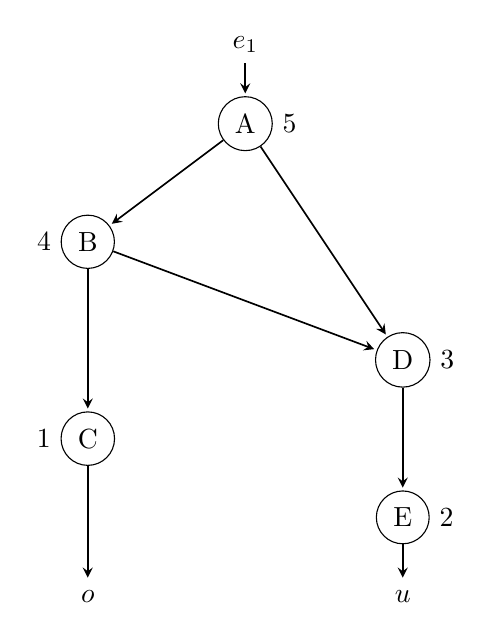
\begin{tikzpicture}
    [pre/.style={<-,shorten <=1pt,>=stealth,semithick}]
    \node (S) at (2,5) {\(e_1\)};
    \node [shape=circle,draw=black] (A) [label=right:5] at (2, 4) {A}
      edge [pre] (S);
    \node [shape=circle,draw=black] (B) [label=left:4] at (0,2.5) {B}
      edge [pre] (A);
    \node [shape=circle,draw=black] (C) [label=left:1] at (0,0) {C}
      edge [pre] (B);
    \node [shape=circle,draw=black] (D) [label=right:3] at (4,1) {D}
      edge [pre] (A)
      edge [pre] (B);
    \node [shape=circle,draw=black] (E) [label=right:2] at (4,-1) {E}
      edge [pre] (D);
    \node (o1) at (0,-2) {\(o\)} edge [pre] (C);
    \node (o2) at (4,-2) {\(u\)} edge [pre] (E);
  \end{tikzpicture}
  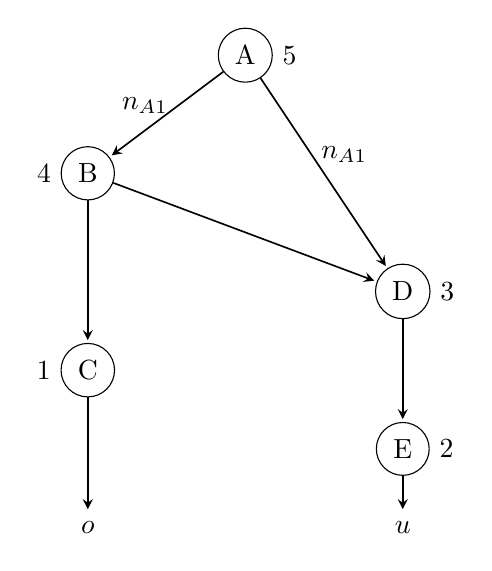
\begin{tikzpicture}
    [pre/.style={<-,shorten <=1pt,>=stealth,semithick}]
    \node [shape=circle,draw=black] (A) [label=right:5] at (2, 4) {A};
    \node [shape=circle,draw=black] (B) [label=left:4] at (0,2.5) {B}
      edge [pre] node[align=left,left,pos=0.6] {\(n_{A1}\)} (A);
    \node [shape=circle,draw=black] (C) [label=left:1] at (0,0) {C}
      edge [pre] (B);
    \node [shape=circle,draw=black] (D) [label=right:3] at (4,1) {D}
      edge [pre] node[align=right,right,pos=0.6] {\(n_{A1}\)} (A)
      edge [pre] (B);
    \node [shape=circle,draw=black] (E) [label=right:2] at (4,-1) {E}
      edge [pre] (D);
    \node (o1) at (0,-2) {\(o\)} edge [pre] (C);
    \node (o2) at (4,-2) {\(u\)} edge [pre] (E);
  \end{tikzpicture}
  \caption{Visualization of a simple asynchronous system with a reversed topological order.}
\label{fig:chap3:sec_sync:visual_dag}
\end{figure}

Figure~\ref{fig:chap3:sec_sync:visual_dag} visualizes a synchronous evaluation Engine.
It shows two DAG representations of an evaluation Engine  where the Nodes A to E are labeled in a reversed topological order and \(o\) and \(u\) represents the output Streams with that name.
The left System is in its initial State and an input Event \(e_1\) is present and can be consumed by the input Node A.
When a Node is chosen to compute by the scheduler, only Node A is enabled, therefore it is scheduled.
The right System is the representation of the next step: Node A has consumed the external Event and produced an internal Event \(n_{A1}\) which is propagated to all it's children: Node B and D.
In the next step Node B would be scheduled, because it has the lowest number of any node that can compute (actually it's the only node that can compute at all, because D has to wait for the event from B).
After B was scheduled, it would have produced the internal Event \(n_{B1}\) which would then be distributed to Nodes C and D.

The complete Run of the synchronous Engine for one Input is the following, where the States are not further defined:

\begin{align*}
  \langle
    (\lambda,                             S_0),
    ((\{ n_{A1}         \}, \{n_{B1}\}),  S_1),
    ((\{ n_{B1}         \}, \{o_1\}),     S_2),\\
    ((\{ n_{A1}, n_{B1} \}, \{n_{D1}\}),  S_3),
    ((\{ n_{D1}         \}, \{u_1\}),     S_4)
  \rangle
\end{align*}

If there were more than one input Event, at this point Node A would be scheduled again.
It would consume the next input and the following Nodes would be scheduled in the same order as before, extending the Run in an obvious way.

\subsection{Asynchronous evaluation}
\label{sec:concepts:behaviour_without_timing:async}

An asynchronous evaluation Engine is one with a fair, but not fixed schedule.

In contrast to the synchronous evaluation Engine it has no fixed schedule, the only requirement is that the schedule is fair.
Therefore predecessors of enabled Nodes can perform multiple computations before their children are scheduled and Events are not \emph{pushed} through the DAG as fast as possible.
\todo{more later}

\section{Equivalence of different schedules without timing functions}
\label{sec:concepts:equivalence_without_timing}

Based on the described behaviours of the approaches we now can proof the equivalence of different Schedules for the same evaluation Engine for a TeSSLa specification.

\begin{lemma}[name = Equivalence of Engines for one Input]\label{lemma:eval_equivalent_if_runs_equal}
  Two evaluation Engines are equivalent for an input, if their Runs are equivalent for that input.
\end{lemma}

\begin{proof}
  Since two Runs are equal if they have the same last State, and all Events which were produced are stored in the State, during both Runs the same output Events had to be generated or else their State would differ.
\end{proof}

As defined by Definition~\ref{def:valid_eval_engine} any evaluation Engine has to be equivalent to a synchronous one to be valid.

The Equivalence is shown in two steps: First in Section~\ref{sec:concepts:equivalence_without_timing:synchronous} it is shown, that all possible synchronous Engines for a specification are equivalent, so there is only one valid Evaluation for a Specification over a fixed Input.
Afterwards in Section~\ref{sec:concepts:equivalence_without_timing:sync_async} it is shown that any asynchronous evaluation Engine is equivalent to a synchronous one.


\subsection{Equivalence of synchronous Systems}
\label{sec:concepts:equivalence_without_timing:synchronous}

When given a series of input Events, two synchronous evaluation Engines for a specification with different schedules will have different Runs.
But both will produce all outputs that can be produced after consuming one specific input before the next Input is consumed as reasoned in Section~\ref{sec:concepts:behaviour_without_timing:synchronous}.
Also both Runs will obviously have the same length (both Engines are the same DAG, so they have the same number of Nodes), let that length be \(l\).

To proof the equivalence of both Engines we can prove the equivalence of their Runs.
To show the equivalence we will show that there is always another Run, which is equivalent to the second one, that has a smaller Distance from the first one.
If such a closer Run always exist, we will show that the Run with Distance \(l, 0\) to the first Run, which has to be the first Run itself, is also an equivalent Run to the second Run.

\begin{theorem}[name = Equivalence of different synchronous evaluation Engines]\label{theorem:equivalence_sync_eval_engines}
  Two synchronous evaluation Engines for a specification with different schedules are equivalent.
\end{theorem}
\begin{proof}

% Let \(\vec{e} = (e_1, e_2, \dots, e_x)\) be the input Events both Engines receive.
Let \(R_1, R_2\) be the Runs of the two Engines for a given TeSSLa specification.
Because each TeSSLa specification contains only a finite amount of Functions and works on finite traces, the Runs also have to be finite.

If the two Runs aren't equal, they must have a Distance which is bigger than \((l, 0)\).
Let \([R_2]\) be the Set of all Runs that are equivalent to \(R_2\).
All of those Runs will also have a Distance from \(R_1\) which is bigger than \((l, 0)\).
Select one Run \(R_2' \in [R_2]\) which has a minimal Distance from \(R_1\).
Let \((d,k) = \delta(R_1, R_2')\).

This means that at Step \(d\) the Run \(R_2'\) has taken a different Transition than Run \(R_1\).
Let the Transitions the Runs have taken be \(\tau_1\) for \(R_1\) and \(\tau_2\) for \(R_2'\).
Run \(R_2'\) will take Transition \(\tau_1\) at step \(d+k\) (as per the definition of the Distance).
Obviously the two Transitions have to be independent of each other, else they couldn't have been taken in different order by the two Runs.

If \(k > 1\) there will be a Transition \(\tau_2' \neq \tau_1\) which is taken by the Run \(R_2'\) at Step \(d+(k-1)\).
While this Transition \(\tau_2'\) must also be taken in the first Run as per Lemma~\ref{lemma:enabled_till_scheduled}, it's not possible, that it was taken before \(\tau_1\), beause than the two runs wouldn't have been the same upto the point where \(\tau_1\) was taken.
Therefore \(\tau_1\) has to be independent of \(\tau_2'\), and because \(\tau_2'\) was scheduled by the second Run before \(\tau_1\) both Transitions are independent of each other.

As of Lemma~\ref{lemma:independent_nodes} which one of them is taken first can't change the enabledness of the Node of the second Transition.
Therefore there is a Run \(R_2''\), which is equal to \(R_2'\), except that the Transitions \(\tau_1, \tau_2'\) are scheduled the other way around.
Figure~\ref{fig:chap3:sec_sync:commutativity_scheduling} visualizes how changing the order of the two Transitions can't change the global State of the Engine after both were taken.
Therefore the Runs \(R_2'\) and \(R_2''\) are equivalent and the Distance to \(R_1\) is \(d, k-1\), which contradicts the initial statement that \(R_1'\) was a Run with a minimal Distance.
This means that there is an equivalent Run to \(R_2\) which has at most the Distance \((d, 1)\).

If \(k = 1\) the Transition \(\tau_2'\) from the previous case is equal to \(\tau_2\).
Based on the same reasoning there also exist a Run \(R_2''\) which is equal to \(R_2'\), except that the order of \(\tau_2\) and \(\tau_1\) is changed, and which is also equivalent to \(R_2'\) and to \(R_2\).
This Run has the Distance \((d, 0)\) from \(R_1\).
This obviously doesn't make sense: The first element of the Distance is the last step where both Runs are equal, the second element describes how many Steps afterwards the differing Transition was taken.
But if it was taken right in the step after the last equal step, there is no difference at that position, so the Difference of \(R_1\) and \(R_2''\) can be at most \((d+1, x), x \in \mathbb{N}_{>0}\).
This also contradicts our initial statement that \(R_2'\) was the Run with the smallest Distance from \(R_1\) which is equivalent to \(R_2\).

Combined we can now say, that there is no lower bound on the Distance of equivalent Runs of \(R_2\) to \(R_1\), therefore the Run with the Distance \((l, 0)\) also has to be equivalent to \(R_2\).

\end{proof}


\begin{figure}
  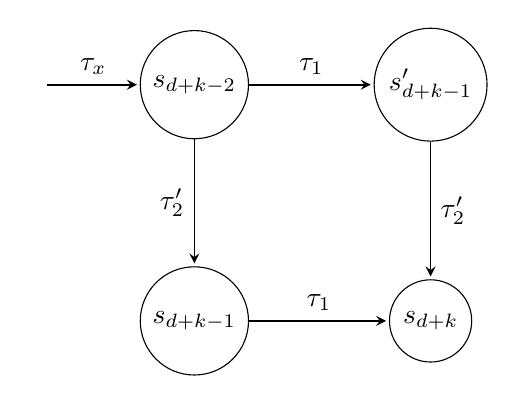
\begin{tikzpicture}
    [pre/.style={<-,shorten <=1pt,>=stealth,semithick}]
    \node (A) at (0,0) {};
    \node [shape=circle,draw=black] (B) at (2, 0) {\(s_{d+k-2}\)}
      edge [pre] node[above] {\(\tau_{x}\)} (A);
    \node [shape=circle,draw=black] (C) at (2, -3) {\(s_{d+k-1}\)}
      edge [pre] node[left] {\(\tau_{2}'\)} (B);
    \node [shape=circle,draw=black] (D) at (5, 0) {\(s_{d+k-1}'\)}
      edge [pre] node[above] {\(\tau_{1}\)} (B);
    \node [shape=circle,draw=black] (E) at (5, -3) {\(s_{d+k}\)}
      edge [pre] node[right] {\(\tau_{2}'\)} (D)
      edge [pre] node[above] {\(\tau_{1}\)} (C);
  \end{tikzpicture}
  \caption{Commutativity Diagramm of Node scheduling}
\label{fig:chap3:sec_sync:commutativity_scheduling}
\end{figure}



\subsection{Equivalence of synchronous and asynchronous schedules}
\label{sec:concepts:equivalence_without_timing:sync_async}

When the Nodes of \(A\) aren't scheduled in reversed topological order, the System can consume inputs before producing all outputs based on the last consumed input.
Therefore the reordering of Runs has to be performed over wider parts of the Run.
% Idea: each step is a commutation of two internal events in regard to the rev top order.
% => show commutativity of traces (note: only valid commutations, no two events, where one depends one the other, can be commuted, this is ensured by the scheduling of nodes that have input buffered)

\section{Behaviour with Timing functions}
\section{Equalitys with Timing functions}
\section{Parallel computation}
 % INCLUDE: concepts
% % !TEX root = ../thesis.tex
%
\chapter{Conclusion}
\label{sec:conclusion}

Citation test~\cite{Pike2010}
 % INCLUDE: conclusion
\cleardoublepage

% --------------------------
% Back matter
% --------------------------
{%
  \setstretch{1.1}
  \renewcommand{\bibfont}{\normalfont\small}
  \setlength{\biblabelsep}{0pt}
  \setlength{\bibitemsep}{0.5\baselineskip plus 0.5\baselineskip}
  \printbibliography[nottype=online]
  \printbibliography[heading=subbibliography,title={Webseiten},type=online,prefixnumbers={@}]
}
\cleardoublepage

\listoffigures
\cleardoublepage

\listoftables
\cleardoublepage

\input{content/colophon}
\cleardoublepage

% !TEX root = ../thesis-example.tex
%
%************************************************
% Declaration
%************************************************
\pdfbookmark[0]{Declaration}{Declaration}
\chapter*{Declaration}
\label{sec:declaration}
\thispagestyle{empty}
\vfill

Ich versichere an Eides statt, die vorliegende Arbeit selbstständig und nur unter Benutzung der angegebenen Quellen und Hilfsmittel angefertigt zu haben.
\bigskip

\noindent\textit{\thesisUniversityCity, \thesisDate}

\smallskip

\begin{flushright}
    \begin{minipage}{5cm}
        \rule{\textwidth}{1pt}
        \centering{\thesisName}
    \end{minipage}
\end{flushright}

%*****************************************
%*****************************************

\clearpage
\newpage
\mbox{}

% **************************************************
% End of Document CONTENT
% **************************************************
\end{document}
